\section{GM-1. Perspectiva del jugador}

\subsection*{Aplicación}

El jugador es el Guardián de la Lluvia: recoge agua en un entorno afectado por contaminantes y acumula una reserva con la que se enfrenta a un OVNI. La recolección tiene dos propósitos: avanzar por puntuación y obtener munición para el combate final. Se pierde al quedarse sin vidas y se gana al derrotar al jefe.

La campaña comprende llanura (niveles 1--10), hielo (11--20) y desierto de Atacama (21--30). El agua normal suma 10 puntos y una carga. Cada 100 puntos permite avanzar; los peligros pueden hacer retroceder. A partir de 3000 puntos comienza el ascenso de tres segundos y después la fase del jefe. \textbf{No existe un nivel numérico 31 jugable}: el jefe es otra fase de la partida y el nivel mostrado permanece en 30.

Noob tiene 5 vidas, Pro 3 y Hacker 1; también cambia el ritmo de caída. Después de cuatro segundos sin recoger agua comienza una reducción progresiva de velocidad, hasta un 60 \%. Agua normal, doble y oasis restablecen la hidratación. No se exige agua durante las rondas de monedas.

{\small
\begin{longtable}{p{0.27\linewidth}p{0.66\linewidth}}
\toprule
Elemento & Efecto base \\
\midrule
\endhead
Agua / agua doble / oasis & +10/+20/+30 puntos y +1/+2/+3 cargas; hidratan \\
Café / fruta & Velocidad $\times$1,5 durante 7 segundos \\
Termo & Protección frente a nieve/hielo durante 8 segundos; elimina esos efectos activos \\
Monedas dobles / puntos dobles & Multiplicador correspondiente durante 8 segundos \\
Sangre / tinta & -20 / -50 puntos \\
Veneno / nieve & -10 / -20 puntos y velocidad a la mitad durante 5 / 4 segundos \\
Hielo / excremento de pájaro & Inmovilización durante 1,5 segundos; hielo también resta 30 puntos \\
Ácido / fuego / cactus & -1 vida y -30/-40/-25 puntos si el golpe es aceptado \\
Bolsa rota & Pierde hasta 5 monedas de la partida y bloquea su recolección durante 4 segundos \\
\bottomrule
\end{longtable}
}

Los puntos nunca quedan negativos. El multiplicador de puntos no multiplica la munición. Tras un daño aceptado hay 1,2 segundos de protección contra nuevos golpes que quitan vida.

El menú ofrece comenzar, tienda, mejores puntuaciones, guía de objetos y versus. Hay 29 aspectos: uno inicial, 15 comprables, nueve por niveles, tres por victoria de campaña y un alien oculto. Son cosméticos. La campaña entrega además una bolsa de 250/400/550 monedas al ganar en Noob/Pro/Hacker. Los récords son locales por dificultad.

Al llegar por primera vez a cada hito 5, 10, 15, 20, 25 y 30 se activa una ronda de monedas de ocho segundos; descender y regresar no permite repetir el mismo hito. Un botón discreto arriba a la izquierda del menú abre otro secreto: combate directo en Pro, con 40 cargas iniciales. Solo desbloquea al alien si se gana y no modifica dinero, ranking ni niveles guardados.

{\small
\begin{longtable}{p{0.2\linewidth}p{0.35\linewidth}p{0.36\linewidth}}
\toprule
Acción & Campaña & Versus local \\
\midrule
\endhead
Movimiento & A/D o flechas izquierda/derecha; ratón/táctil seleccionable & J1 A/D; J2 izquierda/derecha \\
Disparo al jefe & Espacio o clic en el área de juego & J1 W; J2 arriba \\
Pausa & P, Escape o botón & P, Escape o botón \\
Confirmación & Enter o botones & Enter o botones \\
Sonido & M o botón & M o botón \\
\bottomrule
\end{longtable}
}

Versus usa un teclado y pantalla dividida: gana quien sobrevive al rival o vence primero al OVNI, con empate si ambos pierden a la vez o ambos ganan. No altera el perfil de campaña. El control táctil existe, pero no equivale a una validación en Android.

\subsection*{Evidencia}
\begin{itemize}
\item \href{https://github.com/maverick1006/Proyecto-Game-LLuvia-/blob/codex/entrega-final/core/src/main/java/puppy/code/GameLluvia.java#L209}{GameLluvia.java, línea 209} (\texttt{private void menu()})
\item \href{https://github.com/maverick1006/Proyecto-Game-LLuvia-/blob/codex/entrega-final/core/src/main/java/puppy/code/Partida.java#L36}{Partida.java, línea 36} (\texttt{public void actualizar(float delta)})
\item \href{https://github.com/maverick1006/Proyecto-Game-LLuvia-/blob/codex/entrega-final/core/src/main/java/puppy/code/Personaje.java#L78}{Personaje.java, línea 78} (\texttt{public void atrapar(})
\item \href{https://github.com/maverick1006/Proyecto-Game-LLuvia-/blob/codex/entrega-final/core/src/main/java/puppy/code/Dificultad.java#L4}{Dificultad.java, línea 4} (\texttt{NOOB(})
\item \href{https://github.com/maverick1006/Proyecto-Game-LLuvia-/blob/codex/entrega-final/core/src/main/java/puppy/code/Aspecto.java#L4}{Aspecto.java, línea 4} (\texttt{EXPLORADOR(})
\item \href{https://github.com/maverick1006/Proyecto-Game-LLuvia-/blob/codex/entrega-final/core/src/main/java/puppy/code/PartidaVersus.java#L14}{PartidaVersus.java, línea 14} (\texttt{public int getGanador()})
\end{itemize}

\begin{figure}[htbp]
\centering
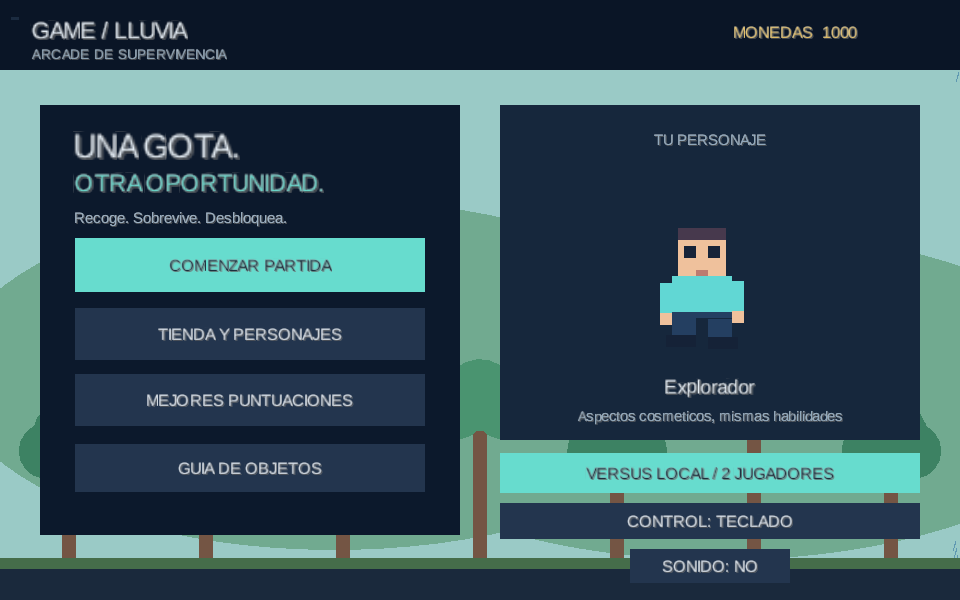
\includegraphics[width=0.95\linewidth,height=0.72\textheight,keepaspectratio]{images/01-menu.png}
\caption{01 menu}
\end{figure}
\begin{figure}[htbp]
\centering
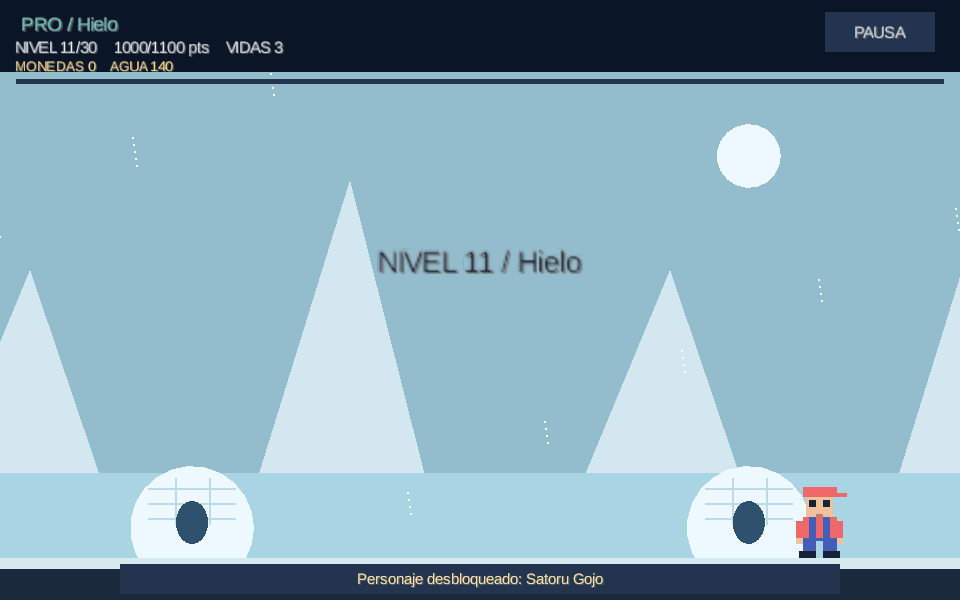
\includegraphics[width=0.95\linewidth,height=0.72\textheight,keepaspectratio]{images/12-hielo.png}
\caption{12 hielo}
\end{figure}
\begin{figure}[htbp]
\centering
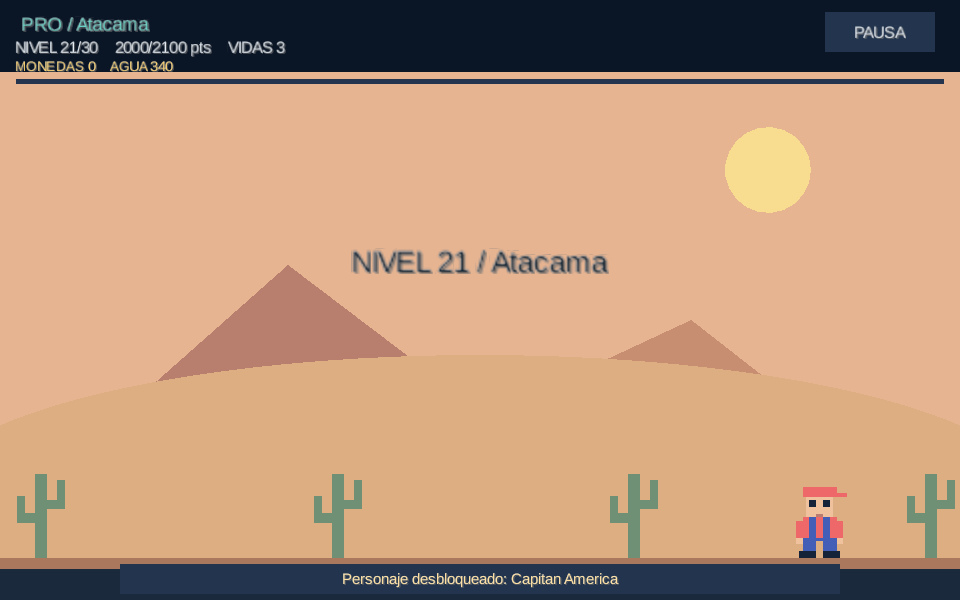
\includegraphics[width=0.95\linewidth,height=0.72\textheight,keepaspectratio]{images/13-atacama.png}
\caption{13 atacama}
\end{figure}
\begin{figure}[htbp]
\centering
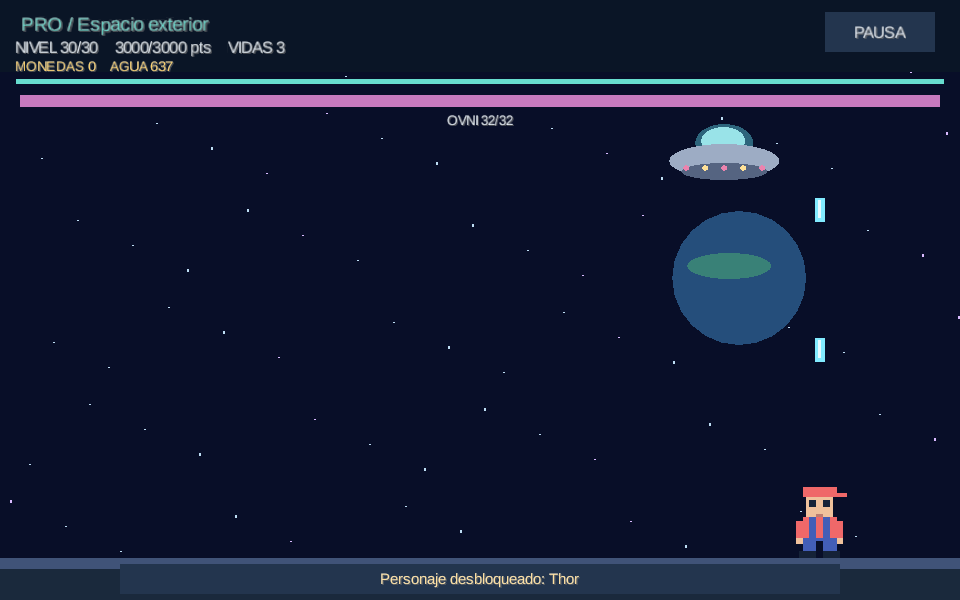
\includegraphics[width=0.95\linewidth,height=0.72\textheight,keepaspectratio]{images/15-jefe.png}
\caption{15 jefe}
\end{figure}
\begin{figure}[htbp]
\centering
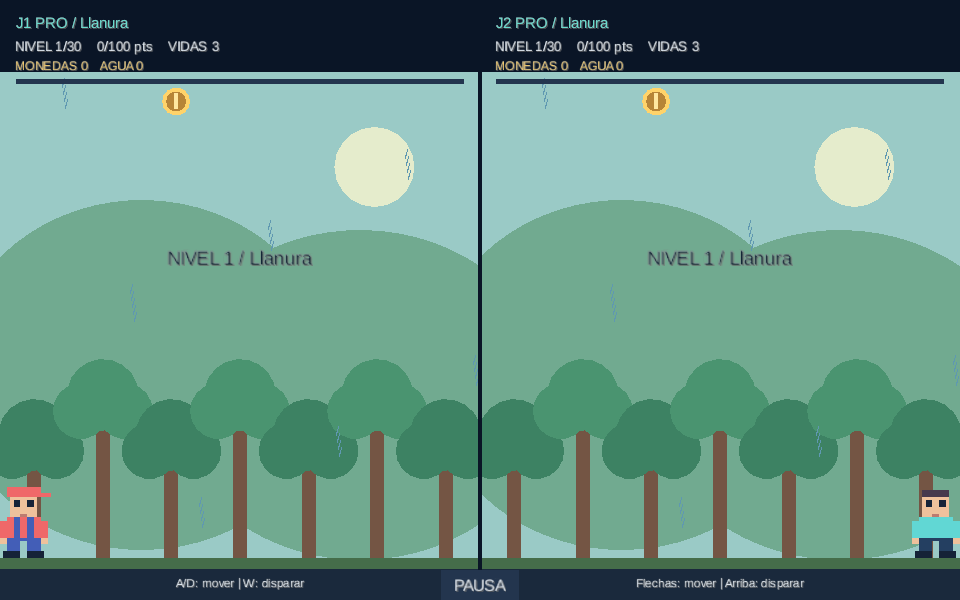
\includegraphics[width=0.95\linewidth,height=0.72\textheight,keepaspectratio]{images/17-versus.png}
\caption{17 versus}
\end{figure}


